\documentclass[letterpaper, 10 pt]{report}

\usepackage{graphicx}
\usepackage{color}
\usepackage{hyperref}
\hypersetup{
    colorlinks,
    linktoc=all,
    citecolor=black,
    filecolor=black,
    linkcolor=black,
    urlcolor=black
}

% -------------------------------------------------------------------------------------
% BEGIN DOCUMENT
% -------------------------------------------------------------------------------------
\begin{document}
\title{User Manual}
\author{Ian George}
\maketitle
\pagestyle{empty}

% -------------------------------------------------------------------------------------
% TABLE OF CONTENTS
% -------------------------------------------------------------------------------------
\tableofcontents
\newpage

% -------------------------------------------------------------------------------------
% INTRODUCTION
% -------------------------------------------------------------------------------------
\section{Schema}
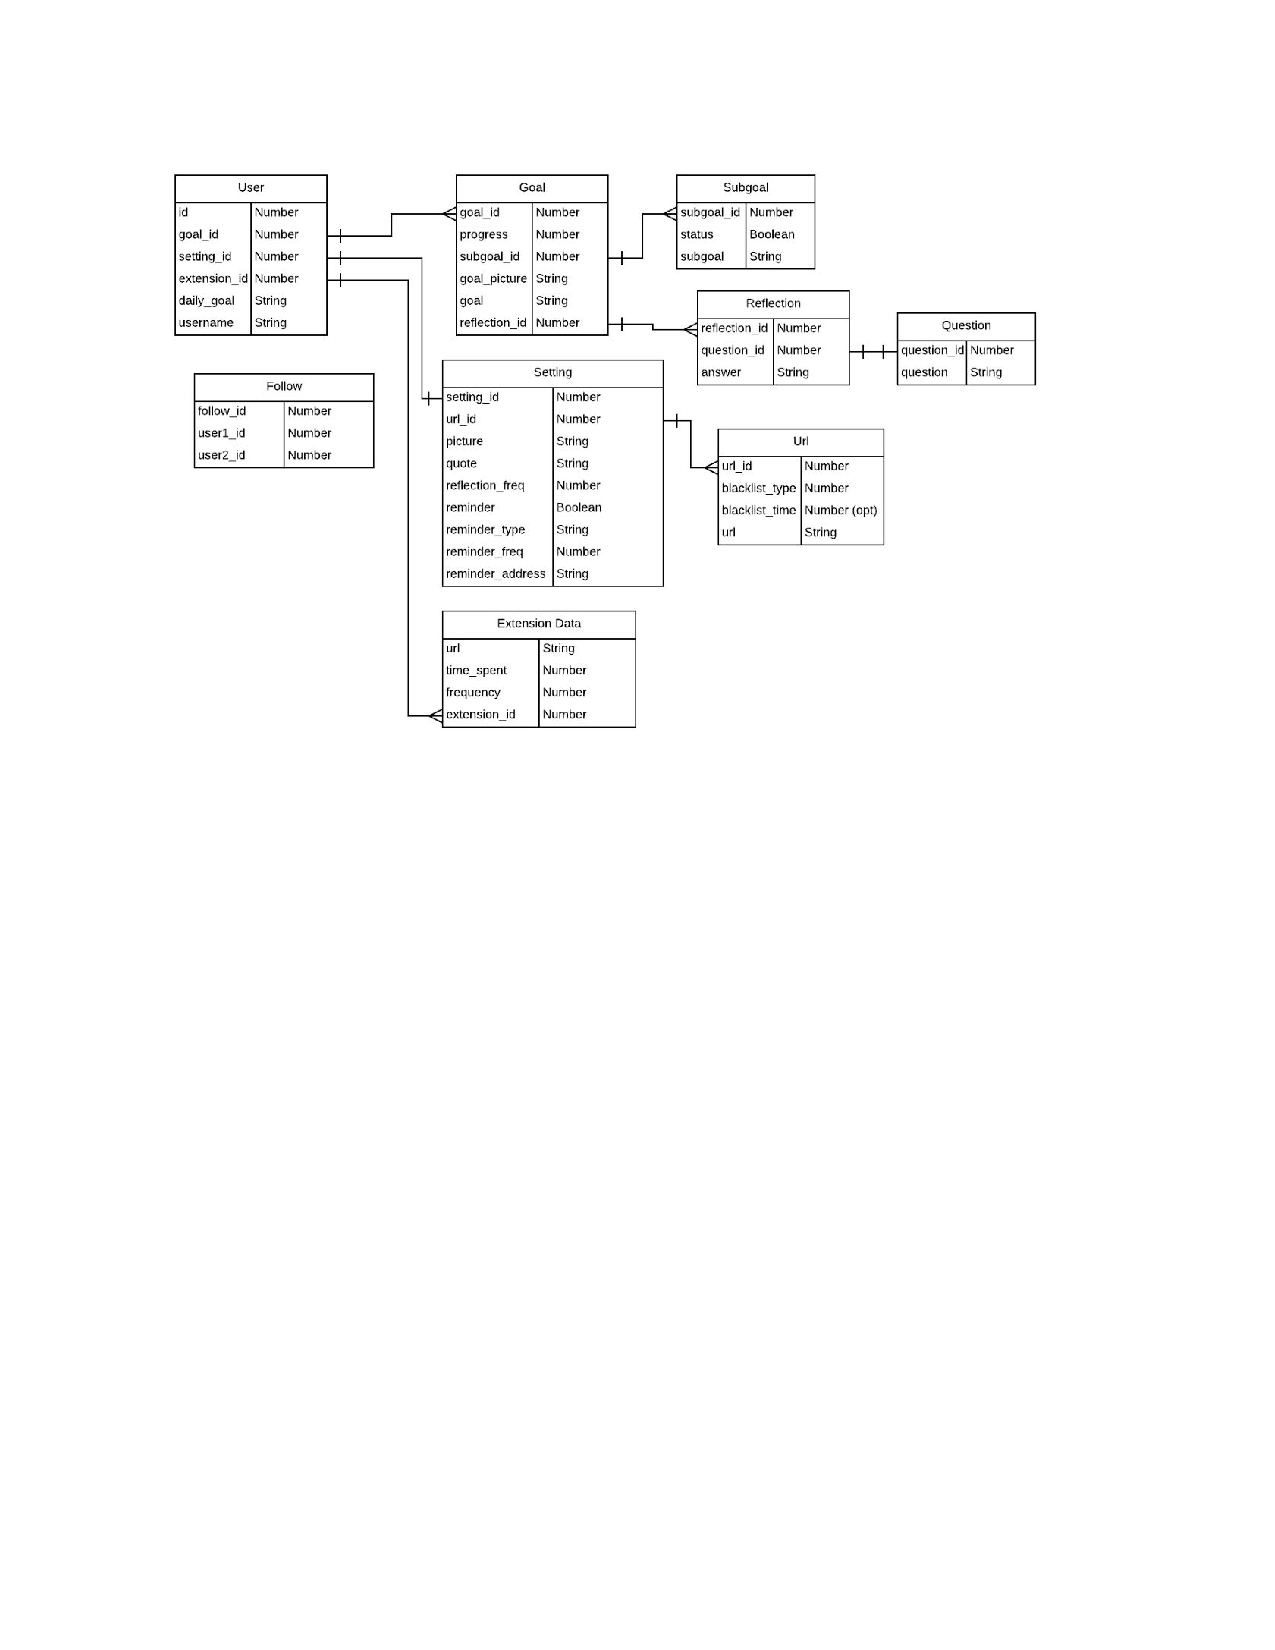
\includegraphics{RelationalData}
\newpage


\section{Front-end}
\subsection{React components}
\begin{itemize}
\item Auth.js: Authentication.
\item Dashboard.js: Dashboard page.
\item Goal.js: AJAX getters and setters on client-sides for goals.
\item Landingpage.js: Initial viewing page for all users.
\item Motivational.js: Handles Inspire Me button.
\item ReflectionQuestion.js: Handles user-submitted reflections in response to displayed questions, extension data. Renders table that forces user to log progress.
\item Selfreflection.js: AJAX client-end getters and setters for reflections.
\item Settings.js: Handles all client-end functions for settings related data-userID, username, blacklisted urls, settings, etc.
\item Sidebar.js: Renders side menu to screen.
\item Site.js: Renders date.
\item Stat.js: Uses recharts to visualize extension data.
\item Subgoal.js: AJAX getters and setters on client-sides for subgoals.
\end{itemize}

\subsection{Middleware}
\begin{itemize}
\item AuthService.js: Handles authentication related middleware functions: getters and setters for tokens, logging in, etc.
\item QuestionSets.js: Dummy questions.
\item SettingsUtil.js: AJAX getter templates.
\end{itemize}

\subsection{Miscallaneous}
\begin{itemize}
\item customJQuery.js: Handles collapsible features.
\item index.js: Gateway, React-GA.
\end{itemize}
\newpage

% -------------------------------------------------------------------------------------
% DAEMONS
% -------------------------------------------------------------------------------------
\section{Back-end}
\subsection{Controllers}
\begin{itemize}
 \item getAllUsers: Obtains all users from the User Schema.
 \item getSingleUser: Obtains specific user from User Schema.
 \item getSettings: Obtains specific user from User Schema, and subsequently obtains settings for that specific user from the Setting Schema.
 \item getBlacklist: Obtains list of blacklisted websites.
 \item getExtension: Obtains specific user from User extension, and using the specific user id, gets Extension data from Extension Schema for that user.
 \item getReflections: Obtains reflections from Reflection Schema.
 \item getAllGoals: Obtains all goals for given user.
 \item getSingleGoal: Obtains single goal for given user.
 \item getSubGoals: Obtains all subgoals for given goal.
 \item getSingleSubgoal: Obtains specific subgoal for given goal.
 
 \item postUser: Inserts new user, with requisite parameters, into User Schema.
 \item postSettings: Inserts new settings for specific user, with requisite parameters into Setting Schema.
 \item postBlackList: Inserts new blacklisted website into Url Schema.
 \item postReflectionId: Inserts new specific reflection by id into Reflection Schema.
 \item postSingleGoal: Inserts new individual goal into Goal Schema for specific User.
 \item postSubGoal: Inserts new individual subgoal into Subgoal Schema for specific Goal.
 
 \item removeSubGoal: Destroys specific individual subgoal in Subgoal Schema.
 \item removeSingleGoal: Destroys specific individual goal in Goal Schema.
 \item removeBlackList: Destroys all blacklists with given id.
 
 \item updateUser: Change daily goal for a given user.
 \item updateUsername: Change username for a given user.
 \item updateSettings: Change settings for a given user.
 \item updateSubgoal: Change given subgoal.
 \item updateSingleGoal: Change given goal.
 \item updateBlacklist: Change blacklisted website.
 \item upsertExtension: Update and insert new extension data for given user.
 
\end{itemize}

\newpage
% -------------------------------------------------------------------------------------
% REFERENCES
% -------------------------------------------------------------------------------------
%\bibliography{}

% -------------------------------------------------------------------------------------
% END DOCUMENT
% -------------------------------------------------------------------------------------
\end{document}